% The poset {a,b,c,d} with a≤b, a≤c≤d drawn as a category (identities shown).
% Source: book/tex/cats/categories.tex (§ Definition and examples).
\documentclass[border=2mm]{standalone}
\usepackage{tikz}
\usetikzlibrary{arrows.meta}
\newcommand{\id}{\mathrm{id}}
\begin{document}
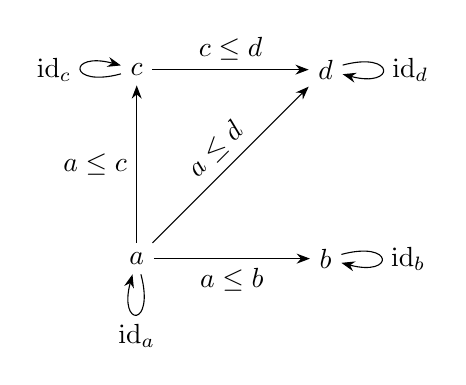
\begin{tikzpicture}[>=Stealth, every loop/.style={min distance=7mm, looseness=12}]
  \node (a) at (0,0) {$a$};
  \node (b) at (2.4,0) {$b$};
  \node (c) at (0,2.4) {$c$};
  \node (d) at (2.4,2.4) {$d$};
  \draw[->] (a)--(b) node[midway,below]{$a\le b$};
  \draw[->] (a)--(c) node[midway,left]{$a\le c$};
  \draw[->] (a)--(d) node[midway,sloped,above]{$a\le d$};
  \draw[->] (c)--(d) node[midway,above]{$c\le d$};
  \draw[->] (a) to[loop below] node[below]{$\id_a$} (a);
  \draw[->] (b) to[loop right] node[right]{$\id_b$} (b);
  \draw[->] (c) to[loop left] node[left]{$\id_c$} (c);
  \draw[->] (d) to[loop right] node[right]{$\id_d$} (d);
\end{tikzpicture}
\end{document}
